%% This work is licensed under the Creative Commons 
%% Attribution-ShareAlike 3.0 Unported License. 
%% To view a copy of this license, visit 
%% http://creativecommons.org/licenses/by-sa/3.0/.

\documentclass{beamer}
\mode<presentation>

\title{\raisebox{-.3\height}{
\includegraphics[width=0.1\textwidth]{images/emacs.pdf}} Emacs: Thou shalt have no other editors}
\author{sciamp [Alessandro Campagni]\\ \texttt{alessandro@lilik.it}}
\date{May 16\textsuperscript{th} 2013\\\raisebox{-.4\height}{
\includegraphics[height=0.1\textwidth]{images/lilik.pdf}} day}

\begin{document}

\begin{frame}
\titlepage
\centering

\includegraphics[height=0.1\textwidth]{images/by-sa.pdf}
\end{frame}

\section{package manager}

\begin{frame}
\frametitle{M-x package-list-packages}
\centering
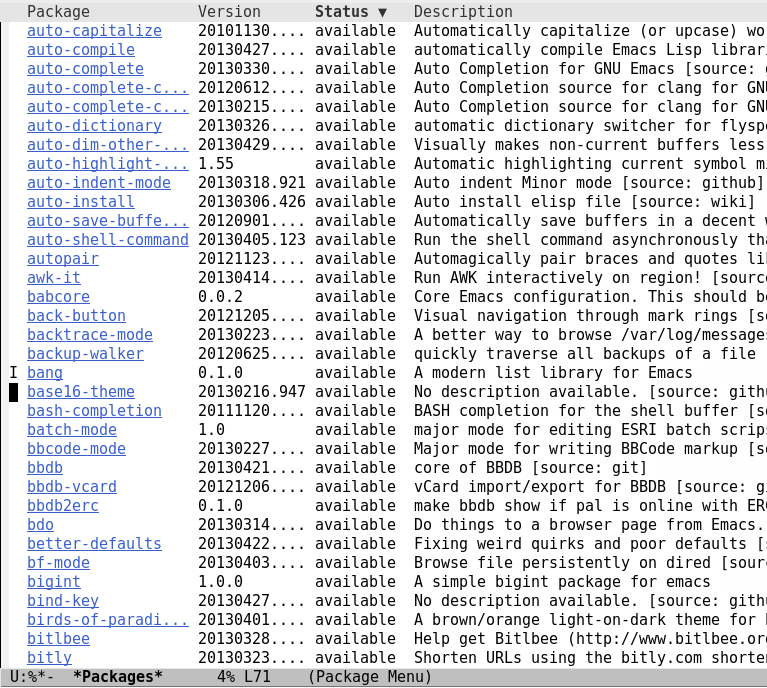
\includegraphics[height=0.8\textheight]{images/package_install.png}
\end{frame}

\subsection{suit up!}

\begin{frame}
\frametitle{Installing Emacs Starter Kit}
\centering
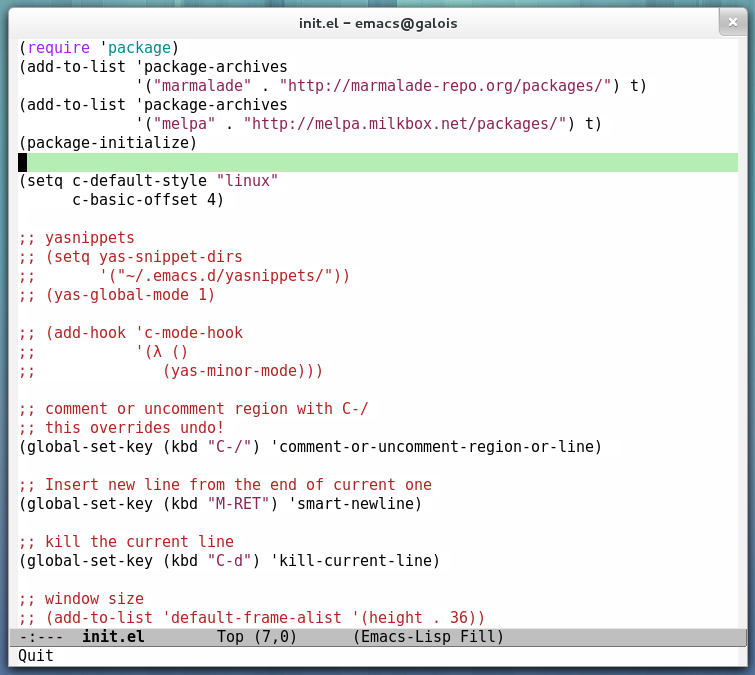
\includegraphics[height=0.8\textheight]{images/emacs_starter_kit.png}
\end{frame}

\section{programming with emacs}

\subsection{code browsing}

\begin{frame}
\frametitle{Emacs code browser}
\centering
\includegraphics<1>[height=0.8\textheight]{images/ecb_default_view.png}
\includegraphics<2>[height=0.8\textheight]{images/ecb_dir.png}
\includegraphics<3>[height=0.8\textheight]{images/ecb_src.png}
\includegraphics<4>[height=0.8\textheight]{images/ecb_methods.png}
\end{frame}

\begin{frame}
\frametitle{Too many source files...}
\begin{columns}[T]
\column{5cm}
\includegraphics<1->[width=\textwidth]{images/ecb_many_files.png}\\
\onslide<2->{just start typing what you're looking for}
\column{5cm}
\includegraphics<3->[width=\textwidth]{images/ecb_file_search.png}
\end{columns}
\end{frame}

\subsection{fancy file opening}
\begin{frame}[t]
\frametitle{Find in repository}
\begin{itemize}[<+->]
\item search files in git/mercurial/bazar/svn... repositories
\item just type the file name (or part of it)
\item \small \texttt{(global-set-key "\textbackslash\,C-x f" 'find-file-in-repository)}
\end{itemize}
\vspace{0.5cm}
\includegraphics<4->[width=\textwidth]{images/find_in_repo_1.png}
\vspace{0.5cm}
\includegraphics<5->[width=\textwidth]{images/find_in_repo_2.png}
\end{frame}

\section{magit: git gets legen - (wait for it) - dary}
\begin{frame}
\frametitle{Magit - git status}
\centering
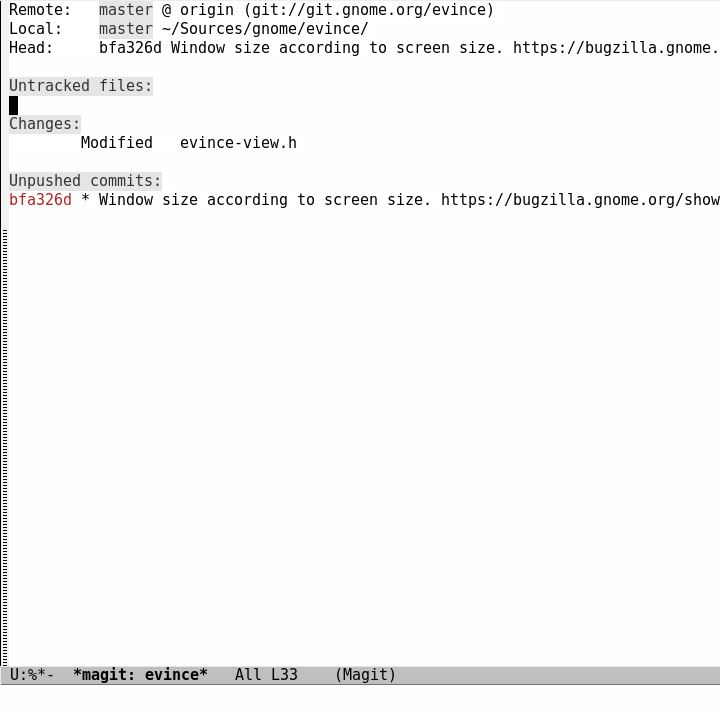
\includegraphics[height=0.9\textheight]{images/magit_status.png}
\end{frame}

\begin{frame}
\frametitle{Magit - diff changes}
\centering
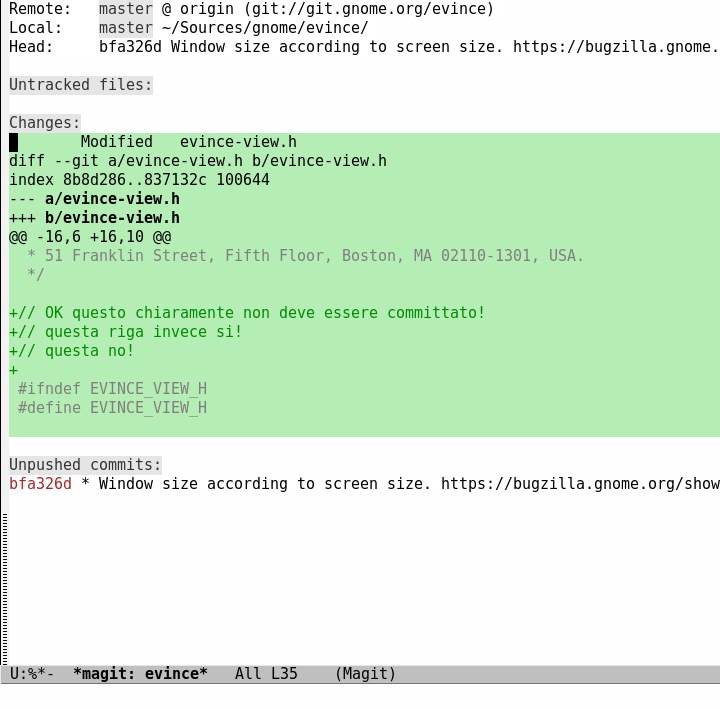
\includegraphics[height=0.9\textheight]{images/magit_show_changes.png}
\end{frame}

\begin{frame}
\frametitle{Magit - staging region}
\centering
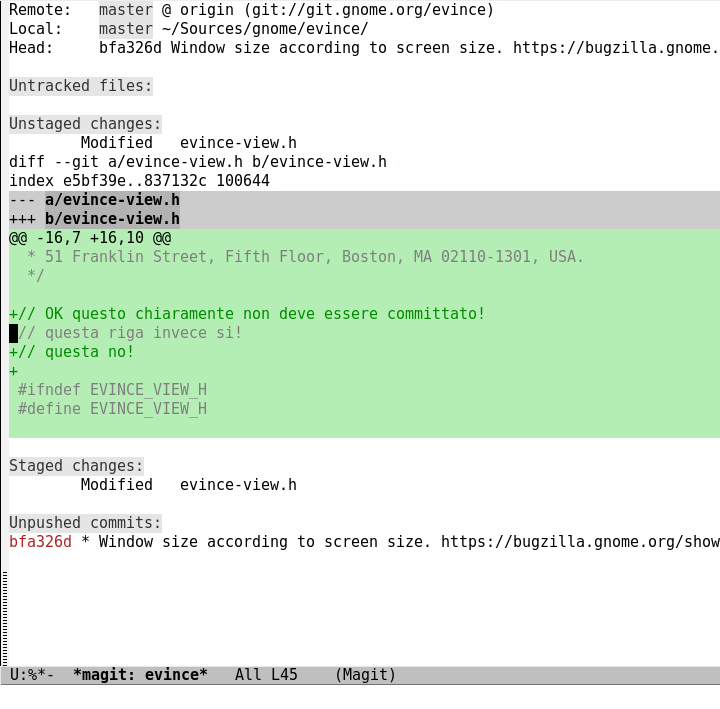
\includegraphics[height=0.9\textheight]{images/magit_staging_region.png}
\end{frame}

\begin{frame}
\frametitle{Magit - staged changes}
\centering
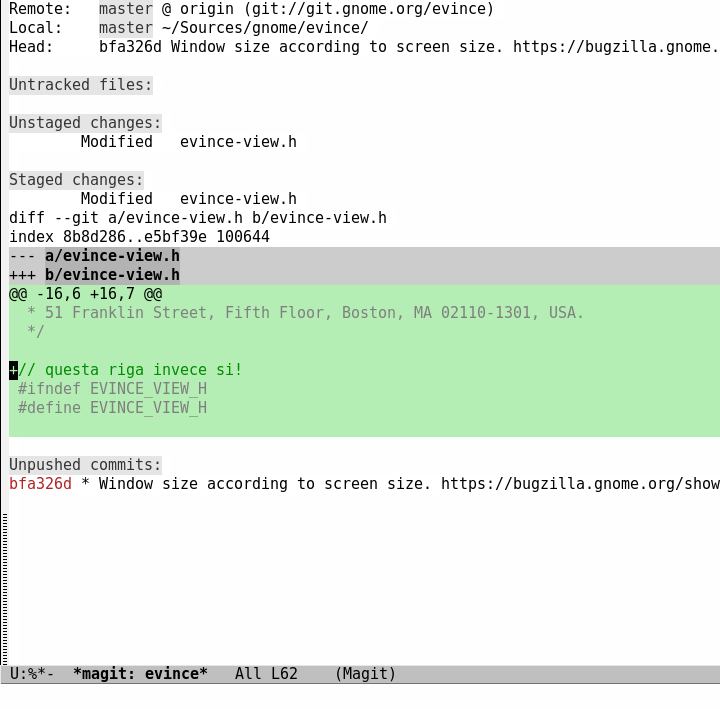
\includegraphics[height=0.9\textheight]{images/magit_staged_changes.png}
\end{frame}

\section{More}
\begin{frame}
\frametitle{Questions?}
\begin{block}{We talked about:}
\begin{itemize}
\item Emacs\\
  \url{www.gnu.org/software/emacs/}
\item Emacs Starter Kit\\
  \url{github.com/technomancy/emacs-starter-kit}
\item Emacs Code Browser\\
  \url{ecb.sourceforge.net/}
\item Find File In Repository\\
  \url{github.com/hoffstaetter/find-file-in-repository}
\item Magit\\
  \url{magit.github.io/magit/}
\end{itemize}
\end{block}
\end{frame}
\end{document}
